\documentclass{article}

% Language setting
% Replace `english' with e.g. `spanish' to change the document language
\usepackage[portuguese]{babel}

% Set page size and margins
% Replace `letterpaper' with `a4paper' for UK/EU standard size
\usepackage[letterpaper,top=2cm,bottom=2cm,left=3cm,right=3cm,marginparwidth=1.75cm]{geometry}

% Useful packages
\usepackage{amsmath}
\usepackage{graphicx}
\usepackage[colorlinks=true, allcolors=blue]{hyperref}

\title{Exercício Programa 02 - Cálculo do Valor de Integral por Monte Carlo}
\author{Alexandre Barsam Junqueira - NºUSP: 12561642}

\begin{document}
\maketitle

\begin{abstract}
Esse relatório busca desenvolver estimativas para o valor de $\int_0^1 f(x) dx$, em que $f(x) = \exp(-ax)\cdot \cos(bx)$ por meio de Simulações de Monte Carlo. Para isso, serão utilizadas quatro técnicas distintas: a) Crude Monte Carlo; b) Hit-or-Miss Monte Carlo; c) Importance Sampling; d) Control Variate. Além disso, busca-se estimar um valor de n para um $erro \leq 0,05\%$.
Observação: nesse documento, considera-se $a=0,16222484$ e $b=0,09532564640$
\end{abstract}

\section{Métodos de Monte Carlo}

Criado por Stanislaw Ulam e John Von Neumann, o Método de Monte Carlo ou Simulação de Monte Carlo é um tipo de algoritmo computacional que utiliza amostragens aleatórias repetidas vezes para obter a probabilidade de um grupo de resultados ocorrer. O método é utilizado, principalmente, como forma de obter aproximações numéricas de funções complexas em que não é viável, ou é mesmo impossível, obter uma solução analítica ou determinística. Dessa forma, consegue-se atuar sobre problemas de otimização e integração numérica, por exemplo.

Na maioria dos casos, as simulações tendem a seguir um padrão:

\begin{enumerate}
    \item Definir um domínio de possíveis entradas;
    \item Gerar entradas randomicamente por meio de uma distribuição probabilística sobre o domínio;
    \item Obter resultados para cada entrada;
    \item Juntar os resultados.
\end{enumerate}

Desse modo, o Método de Monte Carlo é uma ferramenta extremamente poderosa para o entendimento de situações complexas e para aproximações. No entanto, traz consigo problemas relacionados a custo computacional, precisão e dimensionalidade.

\subsection{Crude Monte Carlo}

A ideia básica desse método para integração é aproximar a integral de uma função $f(x)$ em um intervalo $[a, b]$ através da média de valores aleatórios gerados dentro desse intervalo. Suas etapas consistem em:

\begin{enumerate}
  \item \textbf{Gerar números aleatórios}: gera-se $n$ números aleatórios uniformemente distribuídos dentro do intervalo $[a, b]$.
  
  \item \textbf{Avaliar a função nos pontos gerados}: para cada número aleatório gerado, calcular o valor da função $f(x)$ correspondente a esse número.
  
  \item \textbf{Estimar a integral}: a integral da função $f(x)$ no intervalo $[a, b]$ é aproximada multiplicando a média dos valores de $f(x)$ obtidos pelo comprimento do intervalo $[a, b]$.
\end{enumerate}:
\[
\text{Integral} \approx (b - a) \cdot \frac{1}{n} \sum_{i=1}^{n} f(x_i)
\]

Onde:
\begin{itemize}
  \item $n$ é o número de pontos aleatórios gerados.
  \item $x_i$ são os pontos aleatórios gerados dentro do intervalo $[a, b]$.
  \item $f(x_i)$ é o valor da função $f(x)$ avaliada em $x_i$.
  \item $(b - a)$ é o comprimento do intervalo $[a, b]$.
\end{itemize}

\subsubsection{Análise de Variância}
Nesse método de Monte Carlo, a variância é (em que $\gamma$ é o valor real da integral):

\[
\text(\sigma_{c})^2 = \frac{1}{n}\cdot\int_a^b(f(x) - \gamma)^2dx
\]

\subsection{Monte Carlo Hit-or-Miss}

Essa é uma técnica utilizada para calcular integrais definidas através da geração de números aleatórios e da determinação se os pontos gerados estão abaixo ou acima da função que está sendo integrada. Aqui está o processo passo a passo:

\begin{enumerate}
  \item \textbf{Definir uma região em torno da área calculada}: isto é, um retângulo definido pelo intervalo $[a, b]$ no eixo x e pelo intervalo $[0, M]$ no eixo y, onde $M$ é um número suficientemente grande que envolve a função $f(x)$.
  
  \item \textbf{Gerar pontos aleatórios}: gerar um grande número de pontos aleatórios uniformemente distribuídos dentro do retângulo.
  
  \item \textbf{Verificar se os pontos estão abaixo ou acima da função}: para cada ponto gerado $(x_i, y_i)$, verificar se $y_i \leq f(x_i)$ ("hits").
  
  \item \textbf{Calcular a estimativa da integral}: a estimativa da integral da função $f(x)$ no intervalo $[a, b]$ pode ser calculada usando a razão entre o número total de pontos "hits" e o número total de pontos gerados, multiplicado pela área total do retângulo definido pelos intervalos $[a, b]$ e $[0, M]$.
\end{enumerate}

\[
\text{Integral} \approx \frac{\text{hits}}{\text{Total de Pontos}} \cdot (b - a) \cdot M
\]

Onde:
\begin{itemize}
  \item $\text{hits}$ é o número total de pontos que estão abaixo da função $f(x)$.
  \item $\text{Total de Pontos}$ é o número total de pontos gerados.
  \item $[a, b]$ é o intervalo de integração.
  \item $M$ é um número que delimita a função $f(x)$.
\end{itemize}

\subsubsection{Análise de Variância}
Nesse método de Monte Carlo, a variância é (em que $p$ é a proporção real entre a Integral e área do retângulo):

\[
\text(\sigma_{h})^2 = \frac{p(1-p)}{n}
\]

Subtraindo dessa expressão a variância do Crude Monte Carlo, percebe-se que:

\[
\text(\sigma_{h})^2 - (\sigma_{c})^2 = \frac{p(1-p)}{n} -\frac{1}{n}\cdot\int_a^b(f(x) - \gamma)^2dx
\]

\subsection{Importance Sampling}

É uma técnica utilizada para melhorar a eficiência da estimativa de integrais em situações em que o Método de Monte Carlo padrão pode ser ineficiente. Ele funciona selecionando pontos de amostragem de forma não uniforme, priorizando regiões onde a função tem maior contribuição para a integral. Aqui está o processo passo a passo:

\begin{enumerate}
  \item \textbf{Escolher uma distribuição de amostragem}: em vez de amostrar pontos uniformemente dentro do intervalo de integração, escolha uma distribuição de amostragem $g(x)$ que seja relacionada à função $f(x)$ e que enfatize as regiões onde $f(x)$ contribui significativamente para a integral.

  \item \textbf{Transformar a Integral}:
  \[
  \text{$\int_a^b f(x) dx = \int_a^b \frac{f(x)}{g(x)}\cdot g(x)  dx$}
  \]
  
  \item \textbf{Gerar pontos de amostragem}: amostrar pontos de acordo com a distribuição $g(x)$ escolhida. Isso pode ser feito utilizando técnicas como inversão da função de distribuição acumulada ou métodos de amostragem direta.
  
  \item \textbf{Avaliar a função nos pontos de amostragem}: para cada ponto amostrado $x_i$, calcular o valor da função $f(x)$.
  
  \item \textbf{Calcular a estimativa da integral}: a estimativa da integral pode ser calculada utilizando a média ponderada dos valores da função $f(x)$ nos pontos de amostragem, normalizada pela função de densidade de probabilidade $g(x)$:
  
  \[
  \text{Integral} \approx \frac{1}{n} \sum_{i=1}^{n} \frac{f(x_i)}{g(x_i)}
  \]
  
  Onde $n$ é o número total de pontos de amostragem.
\end{enumerate}

\subsubsection{Análise de Variância}
Nesse método de Monte Carlo, a variância é dada por:

\[
\text(\sigma_{s})^2 = \frac{1}{n}\cdot\int_a^b(\frac{f(x)}{g(x)} - \gamma)^2\cdot g(x)dx
\]

Como busca-se $g(x) \propto f(x)$, $\frac{f(x)}{g(x)} \approx constante$, gerando $(\frac{f(x)}{g(x)} - \gamma)^2$ pequeno e tornando a variância menor. Assim, consegue uma variância menor do que a do Crude Monte Carlo.

\subsection{Control Variate}
 Também conhecido com Controle de Variável, envolve a introdução de uma variável adicional (a variável de controle) que está correlacionada com a função a ser integrada, de modo que a variância da estimativa seja reduzida. Além disso, essa nova variável deve ser integrável analitcamente. 

\begin{enumerate}
  \item \textbf{Escolher uma variável de controle}: identifiquar uma variável adicional $\phi(x)$ que esteja correlacionada com a função a ser integrada $f(x)$, onde $x$ é a variável de integração.
  
  \item \textbf{Transformar a Integral}:
  \[
  \text{$\int_a^b f(x) dx = \int_a^b f(x) - \phi(x) + \phi(x)  dx = \int_a^b f(x) - \phi(x) dx + \int_a^b\phi(x)$}
  \]

  \item \textbf{Gerar pontos aleatórios}: gerar um grande número de pontos aleatórios $x_i$ uniformemente no domínio abordado $[a, b]$.

  \item \textbf{Avaliar os pontos em $f(x)$ e $\phi(x)$}: calcular o valor de $f(x_i)$ e $\phi(x_i)$.

  \item \textbf{Calcular a estimativa da integral}: a estimativa da integral pode ser calculada utilizando a seguinte fórmula:]

  \[
  \text{Integral $ \approx \frac{1}{n} \cdot \sum_{i=1}^{n}$} (f(x_i) - \phi(x_i) + \int_a^b\phi(x))
  \]
  
\end{enumerate}

\subsubsection{Análise de Variância}
Nesse método de Monte Carlo, a variância é dada por (em que $\rho$ é a correlação entre as duas funções):

\[
\text(\sigma_{v})^2 = \frac{1}{n}\cdot[\sigma^2(f(x_i)) + \sigma^2(\phi(x_i)) - 2\rho(f(x_i), \phi(x_i))\cdot\sigma(f(x_i))\sigma(\phi(x_i))]
\]

Por esse motivo, quando as $\phi(x)$ aproxima bem $f(x)$, a variância é menor que no Crude Monte Carlo.

\section{Aplicação dos Métodos de Monte Carlo\\ para
$\int_{0}^{1} \exp(-ax)\cdot\cos(bx) dx$}

\subsection{Crude Monte Carlo}

Para a função abordada, tem-se que:
\[
\text{$\int_0^1 f(x) dx$} \approx \frac{1}{n} \sum_{i=1}^{n} f(x_i)
\]

O resultado ($r$) com $n = 5\cdot10^6$ foi: $r = 0,921793085$.

\subsection{Monte Carlo Hit-or-Miss}

Com a função fornecida, obtém-se $[a,b] = [0, 1]$ e $M = 1$:
\[
\text{$\int_0^1 f(x) dx$} \approx \frac{\text{hits}}{\text{Total de Pontos}}
\]
O valor de $M=1$ pode ser utilizada, pois, nesse intervalo, a função se comporta segundo a Figura 1 (sendo seu valor máximo em $x = 0$ com $f(x) = 1$).

\begin{figure}[h]
\centering
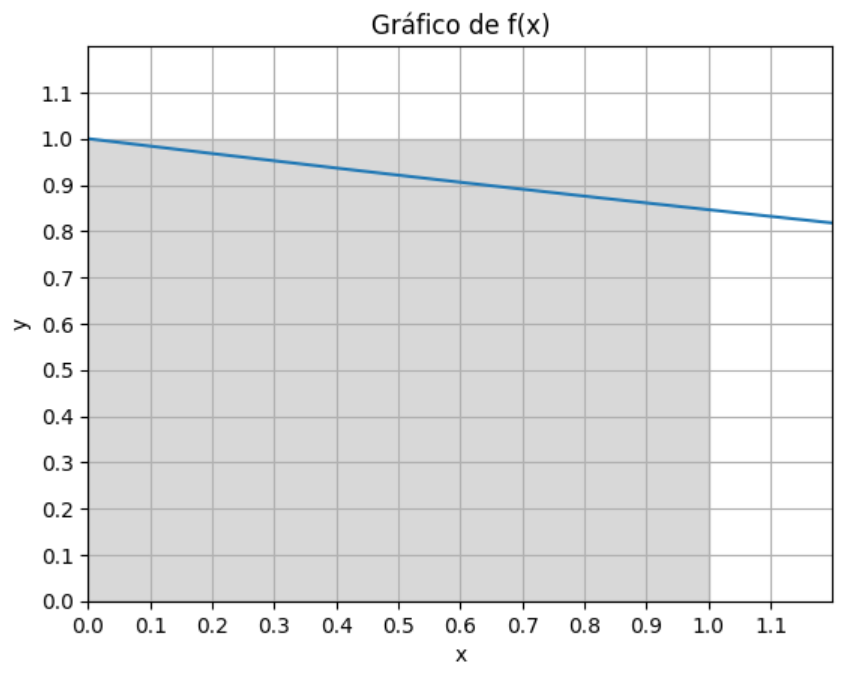
\includegraphics[width=0.50\linewidth]{Gráfico f(x).png}
\caption{\label{fig:Gráfico 1} Comportamento de f(x)}
\end{figure}

O resultado ($r$) com $n = 5\cdot10^6$ foi $r = 0.9216554$.

\subsection{Importance Sampling}

Para a definição de qual distribuição $g(x)$ utilizar, serão analisadas as distribuições Beta, Gamma e Weibull. As funções densidade de probabilidade (PDF) de cada uma são:
\[ h_{beta}(x;\alpha,\beta) = \frac{x^{\alpha-1}(1-x)^{\beta-1}}{B(\alpha,\beta)} \]
\[ h_{gamma}(x;k,\theta) = \frac{1}{\theta^k \Gamma(k)} x^{k-1} e^{-\frac{x}{\theta}} \]
\[ h_{weibull}(x;k,\lambda) = \frac{k}{\lambda} \left(\frac{x}{\lambda}\right)^{k-1} e^{-(x/\lambda)^k} \]

Com o intuito de que essas distribuições se apliquem a um domínio $[a, b]$, deve-se modificar as funções. Dada uma distribuição $g(x)$ com densidade acumulada (CDF) $H(x)$, então $G(x) = \frac{H(x) - H(a)}{H(b) - H(a)}$ é uma densidade acumulada definida em [a,b]. Para $[0, 1]$, $G(x) = \frac{H(x)}{H(1)}$. Assim, derivando ambos lados: $g(x) = \frac{h(x)}{H(1)}$. Por isso, as fórmulas utilizadas serão:
\[ g_{beta}(x;\alpha,\beta) = \frac{h_{beta}(x;\alpha,\beta)}{H_{beta}(1;\alpha,\beta)} \]
\[ g_{gamma}(x;k,\theta) = \frac{h_{gamma}(x;k,\theta)}{H_{gamma}(1;k,\theta)} \]
\[ g_{weibull}(x;k,\lambda) = \frac{h_{weibull}(x;k,\lambda)}{H_{weibull}(1;k,\lambda)} \]

Como mencionado anteriormente, a função $g(x)$ será mais efetiva se proporcional à função $f(x)$. Por isso vale otimizar os parâmetros de cada uma das funções abordadas. Para isso, pode-se utilizar tanto um guia visual, como também buscar por parâmetros que minizem as diferenças entre as funções. Nesse artigo, buscou-se minimizar o RMSE (\textit{Root Mean Square Error}) ao utilizar otimização de \textit{least square}. Realizando esse procedimento várias vezes, os valores médios encontrados são:

\[ \alpha = 0,972 \]
\[ \beta = 1,016 \]
\[ k_{gamma} = 1,000 \]
\[ \theta = 6,475 \]
\[ k_{weibull} = 1,000 \]
\[ \lambda = 6,488 \]

Além disso, verificou-se que a distribuição Gamma e Weibull obtiveram um RMSE menor que a Beta. No entanto, essa diferença foi pequena: $RMSE_\beta = 0.07932$; $RMSE_\gamma=0,07823$ e $RMSE_w = 0,07823$.

Com isso, pode-se construir cada uma das distribuições e, assim, amostrar pontos de acordo com a distribuição por meio de amostragem direta. Por fim, basta realizar o cálculo:

  \[
  \text{Integral} \approx \frac{1}{n} \sum_{i=1}^{n} \frac{f(x_i)}{g(x_i)}
  \]

Os resultados para cada distribuição foram: $r_{beta} = 0,921758$; $r_{gamma} = 0,921766$; $r_{weibull} = 0.921764$.

\subsection{Control Variate}

Por fim, no método de variável de controle, foi utilizada uma equação polinomial $p(x)$ que aproxima-se $f(x)$ no intervalo $[0, 1]$. Para construir o polinômio, utilizou-se a Série de Taylor
\[
f(x) = \sum_{n=0}^{\infty} \frac{f^{(n)}(x_0)}{n!}(x - x_0)^n
\]
cujo resto é dado por
\[
R_n(x) = \frac{f^{(n+1)}(\xi)}{(n+1)!}(x - x_0)^{n+1}
\]

Primeiramente, definiu-se $x_0 = 0,5$, por ser o ponto médio do domínio $[0, 1]$. Além disso, realizou-se a expansão de taylor somente até o segundo termo, visto que o resto já estava extremamente baixo. Assim, a aproximação ficou da seguinte forma:

\[
p(x) = f(x_0) + f'(x_0)\cdot(x - x_0) \approx 0,921 + 0,153\cdot(x-x_0)
\]

em que $f'(x) = -a\cdot\exp(-ax)\cdot\cos(bx) - b\cdot\exp(-ax)\cdot\sin(bx)$. Por sua vez, o erro é dado por:

\[
R_1(x) = \frac{f''(\xi)}{2}\cdot(x - x_0)^2
\]

em que $f''(x) = (a^2 - b^2)\cdot\exp(-ax)\cdot\cos(bx) + 2ab\cdot\exp(-ax)\sin(bx)$. Para verificar o maior erro possível no domínio $[0, 1]$, deve-se maximizar $f''(\xi)$ e $(x-x_0)^2$. Os valores encontrados são: $\xi \approx 0,241$ e $x = 0$ ou $x = 1$, resultando em $R_1(x) \approx 2,16\cdot10^{-3}$. Ademais, a correlação entre $f(x)$ e $p(x)$ calculada foi de $corr\approx1$.

\begin{figure}[h]
\centering
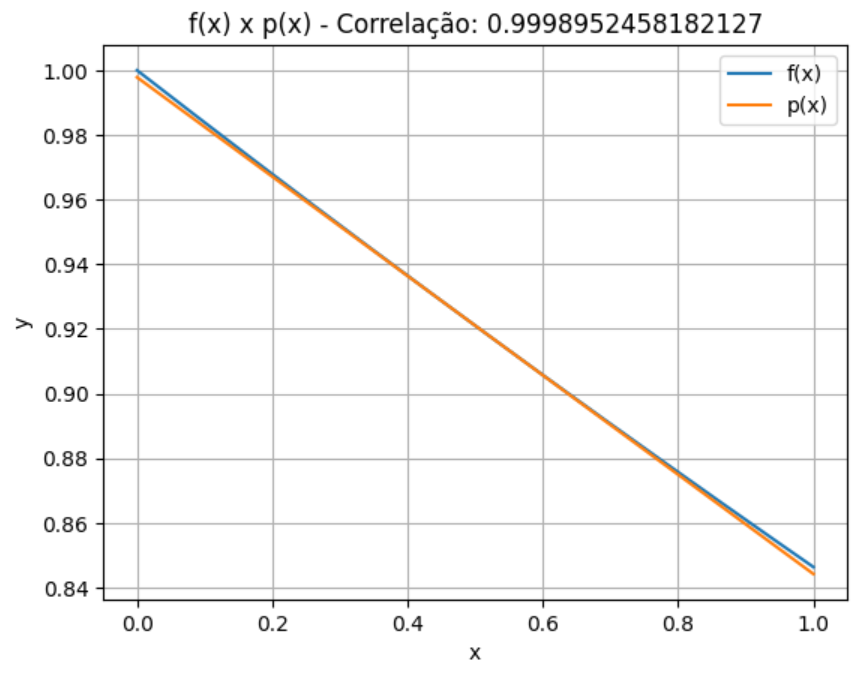
\includegraphics[width=0.50\linewidth]{f(x) x p(x).png}
\caption{\label{fig:Gráfico 2} Semelhança entre f(x) e p(x)}
\end{figure}

Por fim, tem-se que:

  \[
  \text{Integral $ \approx \frac{1}{n} \cdot \sum_{i=1}^{n}$} (f(x_i) - \phi(x_i) + \int_0^1p(x))
  \]

com $\int_0^1p(x) = 0,92104$. Desse modo, basta gerar $x_i$ aleatórios uniformemente em $[0, 1]$, chegando ao resultado $r = 0,92176132$.

\section{Valor de $n$}
Com o intuito de determinar um valor de $n$ que estime com precisão de 0,05\% o valor da integral com uma confiança de 95\%, basta utilizar um intervalo de confiança construído à partir da da variância de cada método. No entanto, como abordado, a variância do Método Hit-or-Miss é sempre maior que a do método Crude Monte Carlo, que por sua vez é maior que a variância tanto do Importance Sampling quanto do Control Variate.

Portanto, ao encontrar um $n$ que satisfaça essa condição para o Hit-or-Miss, sabe-se que esse valor consegue prever o valor da estimar com precisão de 0,05\% o valor da integral com uma confiança maior que 95\%.

Por sua vez, o intervalo de confiança do Hit-or-Miss é:
$$IC_h = \left[integral_a - z \cdot \sqrt{\frac{p_a \cdot (1 - p_a)}{n}}, integral_a + z \cdot \sqrt{\frac{p_a \cdot (1 - p_a)}{n}}\right]$$

Definindo-se a margem de erro como metade do tamanho do intervalo de confiança, tem-se que: $$e = z_\rho \cdot \sqrt{\frac{p_a (1 - p_a)}{n}}$$ $$n = \left(\frac{z_\gamma}{e}\right)^{2}  p_a \cdot (1 - p_a)$$

Ao buscar uma confiança de 95\% e $e = 0,05\%$, $z_\rho\apporx1,96$ e, no pior dos casos, $p_a=0,5$ (pois maximiza o valor da função). Alternativamente, utilizando a estimativa do Crude Monte Carlo, $p_a = 0,921793085$. Com isso:
$$n_{max} = 3.841.600$$
$$n_{estimativa} = 1.107.773$$

Assim, com esse valor de $n$, sabe-se que é possível obter uma precisão de 0,05\% nas estimativas com confiança $\pho \geq 95\%$ para todos os métodos abordados.

\section{Distribuições Beta, Gamma e Weibull}
Aqui estão as distribuições segundo os parâmetros encontrados no artigo:

\begin{figure}[h]
\centering
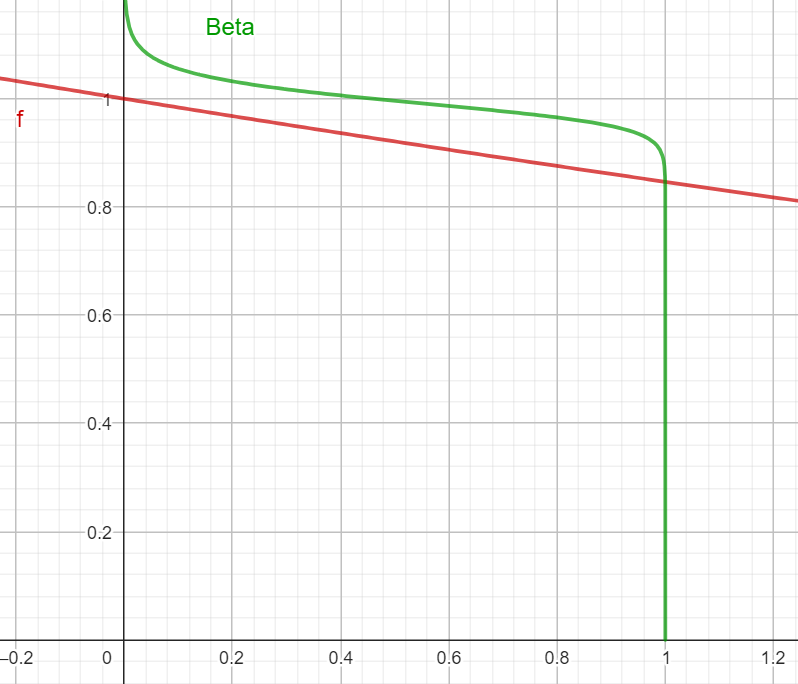
\includegraphics[width=0.60\linewidth]{Beta.png}
\caption{\label{fig:Figura 4}Distribuição Beta.}
\end{figure}
\begin{figure}[h]
\centering
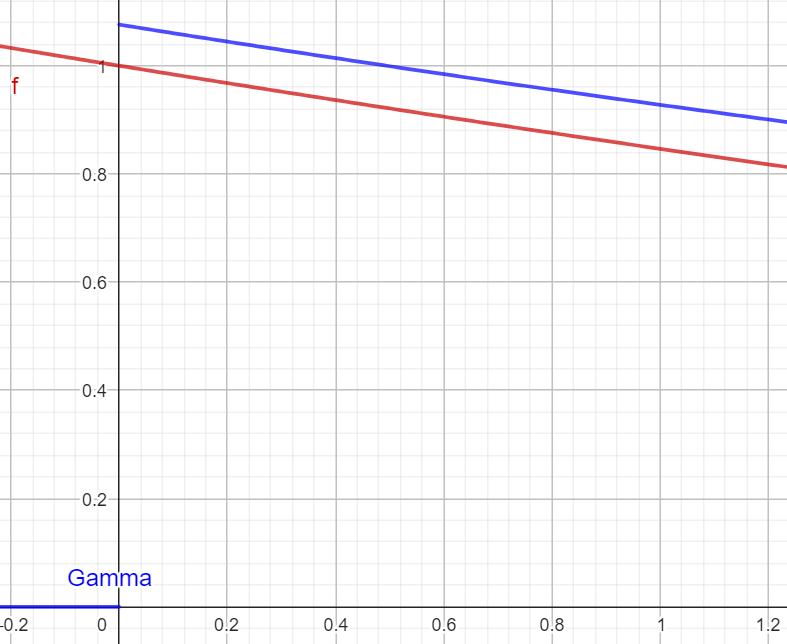
\includegraphics[width=0.60\linewidth]{Gamma.png}
\caption{\label{fig:Figura 4}Distribuição Gamma.}
\end{figure}
\begin{figure}[h]
\centering
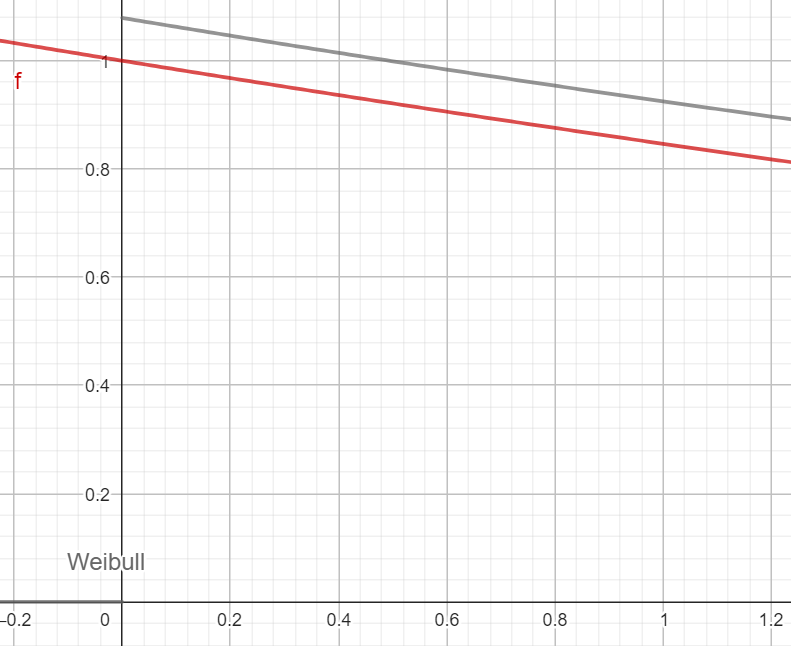
\includegraphics[width=0.60\linewidth]{Weibull.png}
\caption{\label{fig:Figura 4}Distribuição Weibull.}
\end{figure}

Visualmente, percebe-se que, de fato, as distribuições são praticamente proporcionais a $f(x)$, especialmente no caso da Gamma e da Weibull. Por sua vez, a distribuição beta tem um encaixe pior (relativamente proporcional no meio do intervalo, porém com distorções perto de 0 e 1), o que justifica seu RMSE maior que o das outras distribuições.

\end{document}